\documentclass[11pt]{article}
\usepackage[margin=1in]{geometry}
\usepackage{amsmath,amssymb,amsthm}
\usepackage{graphicx}
\usepackage{booktabs}
\usepackage{caption}
\usepackage[hidelinks]{hyperref}
\usepackage{xcolor}
\usepackage{enumitem}
\setlist{nosep,leftmargin=1.4em}
\graphicspath{{../figures/}}
\newtheorem{theorem}{Theorem}
\newtheorem{proposition}{Proposition}
\newtheorem{definition}{Definition}
\captionsetup{font=small,labelfont=bf}
\renewcommand{\topfraction}{0.9}\renewcommand{\bottomfraction}{0.8}\renewcommand{\textfraction}{0.07}\renewcommand{\floatpagefraction}{0.75}

\title{\textbf{Where Should the Defibrillators Go?}\\[0.3em]
\large Survival-Based, Opening-Hours-Aware and Fairness-Constrained AED Placement\\ from Open Data in Virginia Beach}
\author{Aryan Padarthi\\ \small EurekaDev 2026 --- Research Track, Math \& Physics}
\date{October 2026}

\begin{document}
\maketitle

\begin{abstract}
\noindent
Out-of-hospital cardiac arrest (OHCA) kills about nine in ten of the roughly 137{,}000 patients reported to the U.S. CARES registry each year, and every minute without defibrillation lowers the chance of survival. Public automated external defibrillators (AEDs) can close that gap, but only if they are placed where arrests happen, \emph{and} can be reached when they happen. Using a public data set of 2{,}706 cardiac arrests in Virginia Beach, Virginia (2017--2019), a 52{,}708-node walking network, 929 candidate host sites with opening hours from OpenStreetMap, and the CDC Social Vulnerability Index, we formulate AED placement as an expected-survival facility-location problem, prove that its objective is monotone submodular (so a greedy algorithm is guaranteed $\ge 63\%$ of optimal; in practice it reached $\ge 99.9\%$), and solve it exactly as a mixed-integer program. In five-fold temporal cross-validation with address-clustered confidence intervals, our model achieves 42--67\% more out-of-sample expected survival gain than the standard maximal covering model for 25--200 AEDs, beats it in all 30 robustness checks, and also beats stronger baselines from the literature. Planning as if AEDs were reachable 24/7 overstates their real benefit by 67--106\%, and housing AEDs in outdoor 24/7 cabinets yields 41--63\% more benefit, so one cabinet is worth about two indoor AEDs. We test, and reject, the hypothesis that AEDs should follow historically slow EMS: location explains only 7\% of the variation in response time. This motivates a model that needs only a city's response-time \emph{distribution}, and yields a derived ``reach curve'': an AED loses half its value within about 123 m of walking. Finally, a fairness floor across vulnerability quartiles has no detectable out-of-sample cost, and a simple bound shows that full parity is unreachable with building-hosted AEDs alone.
\end{abstract}

\section{Background \& Problem Definition}

\paragraph{Clinical urgency and defibrillation delays.} In the United States, emergency responders treated roughly 137{,}000 non-traumatic out-of-hospital cardiac arrests reported to the CARES registry in 2024 (a registry covering about 186 million people), but only 10.5\% of those patients survived to leave the hospital alive \cite{cares2024}. For patients in ventricular fibrillation or pulseless ventricular tachycardia, survival hinges on delivering an electric countershock before irreversible ischemic injury takes hold. Every minute of delay causes a steep survival drop: in King County, Washington, predicted survival fell by 2.3 percentage points for every minute until CPR began, and by another 1.1 points for each minute of delay to defibrillation \cite{larsen1993}.

\paragraph{Bystander intervention and physical access barriers.} Automated external defibrillators (AEDs) allow lay bystanders to deliver early shocks guided by voice prompts. When a bystander applies an AED before EMS arrives, survival more than doubles: 24\% versus 9\% for bystander CPR without an AED in the Resuscitation Outcomes Consortium \cite{weisfeldt2010}, and 66.5\% versus 43.0\% for observed public shockable arrests (adjusted odds ratio 2.62) \cite{pollack2018}. Yet bystanders attach an AED in only 12.6\% of public arrests nationwide \cite{cares2024}. In practice, bystanders face two basic physical barriers: the nearest unit is too far to walk to, or it sits behind locked doors in a building closed for the evening or weekend \cite{hansen2013,karlsson2019,deakin2018}.

\paragraph{Study setting: Virginia Beach.} Virginia Beach offers an unusual opportunity to study these spatial-temporal dynamics. Spanning roughly 460{,}000 residents across high-density coastal corridors, sprawling suburbs, and rural agricultural land, it is one of very few U.S. jurisdictions that publish complete, incident-level cardiac arrest records with the precise EMS response time for each dispatch \cite{custodio2022}. Across these records, the median time from the 911 call to the first unit's arrival is 7.2 minutes, and 41\% of patients waited longer than 8 minutes (Figure~\ref{fig:rt})---an interval where an accessible public AED could mean the difference between life and death.

\paragraph{Research questions.} Given a municipal budget of $p$ AEDs and a set of candidate host facilities, we examine four core questions:
\begin{enumerate}
\item[\textbf{RQ1}] Does optimizing site selection for \emph{expected survival} over actual walking networks yield greater benefit on held-out arrests than standard models that maximize historical arrests covered within a fixed 100-meter buffer?
\item[\textbf{RQ2}] How severely does the assumption of continuous 24/7 building access inflate projected survival gains, and what share of that lost benefit can outdoor 24/7 smart cabinets recover?
\item[\textbf{RQ3}] Can historical ambulance delays guide prospective placement, or is dispatch latency too spatially variable to predict where AEDs will be needed next?
\item[\textbf{RQ4}] What is the price of fairness when requiring every social vulnerability quartile to receive an equitable share of expected survival, and does candidate site density impose a hard mathematical ceiling on parity?
\end{enumerate}

\begin{figure}[htbp]
\centering
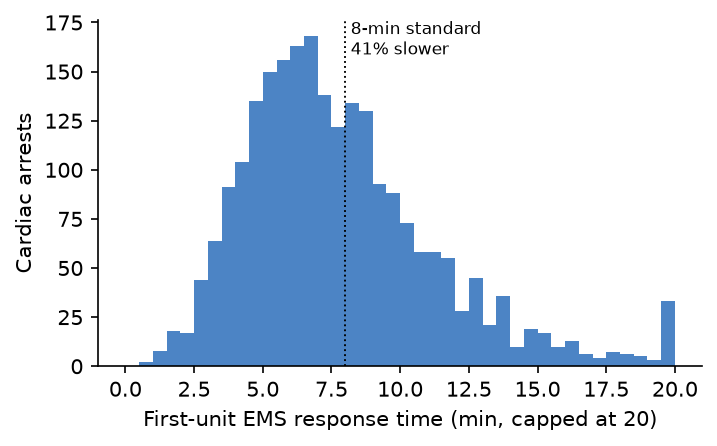
\includegraphics[width=0.48\linewidth]{fig2_response_times.png}\hfill
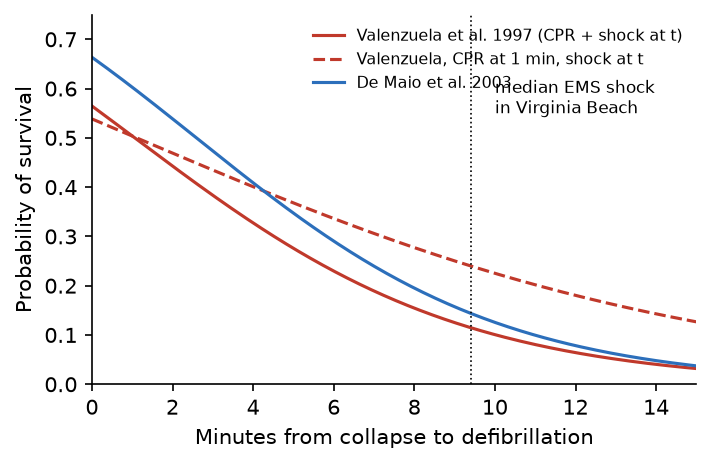
\includegraphics[width=0.48\linewidth]{fig1_survival.png}
\caption{\textbf{Left:} first-unit EMS response times for the 2{,}332 Virginia Beach arrests with a recorded time. \textbf{Right:} the two published survival curves used in this study \cite{valenzuela1997,demaio2003,erkut2008}. A shock at the median Virginia Beach EMS time (dotted line) gives far lower survival than a shock in the first few minutes. Valenzuela's curve is measured from collapse; De Maio's from the 911 call.}
\label{fig:rt}
\label{fig:survival}
\end{figure}

\section{Literature Review}

\paragraph{Survival and time.} The link between time and survival is among the best-established facts in resuscitation science. Larsen et al.\ fit a linear model to 1{,}667 witnessed ventricular-fibrillation arrests and found that predicted survival falls from 67\% by 2.3, 1.1 and 2.1 percentage points for every minute of delay to CPR, defibrillation and advanced life support, respectively \cite{larsen1993}. Valenzuela et al.\ replaced this with a logistic model that depends only on the collapse-to-CPR and collapse-to-shock intervals and generalizes across U.S. cities \cite{valenzuela1997}. De Maio et al.\ fit a similar curve to EMS response time for all treated arrests in Ontario \cite{demaio2003}. Erkut, Ingolfsson and Erdo\u{g}an showed that replacing yes/no ``coverage'' with such survival functions changes, and improves, where ambulances should be based \cite{erkut2008}; we use their published forms of both curves.

\paragraph{Bystander AEDs work, but are rarely used.} Weisfeldt et al.\ found that an AED was applied before EMS arrival in only 2.1\% of 13{,}769 arrests, but that its use raised survival (adjusted OR 1.75) \cite{weisfeldt2010}. Pollack et al.\ found that the benefit of a bystander shock ``increased progressively as EMS response time became longer'' \cite{pollack2018}, and Hindborg et al.\ found a significant survival benefit specifically when EMS took 7--9 minutes in public arrests \cite{hindborg2025}. These findings motivate RQ3.

\paragraph{Access in space and time.} Copenhagen data showed that 61.8\% of public arrests happen in the evening, at night or on weekends, while only 9.1\% of AEDs were accessible 24/7; limited hours cut coverage by 53.4\% during those periods \cite{hansen2013}. When the nearest AED was accessible, 30-day survival was 28.8\% versus 16.4\% when it was not \cite{karlsson2019}. In England, only 34.3\% of AEDs were available at night \cite{deakin2018}. Walking routes matter too: switching from straight-line to route distance cut 100-metre coverage from 24.2\% to 9.5\% in Copenhagen \cite{karlsson2021}.

\paragraph{Optimization models.} Toregas et al.\ introduced the location set-covering problem \cite{toregas1971} and Church and ReVelle the \emph{maximal covering location problem} (MCLP): place $p$ facilities to cover as much demand as possible within a fixed distance \cite{church1974}. A 2025 scoping review of 43 AED-placement studies found the MCLP to be the most common model \cite{petravic2025}. Chan et al.\ first applied optimization to AED siting in Toronto, using historical arrests and a 100-metre radius \cite{chan2013,chan2016}. Sun et al.\ added time-of-day availability and found that assuming 24/7 access overstated coverage by 21.5\% \cite{sun2016}; an \emph{in silico} trial in Copenhagen found optimized placement covered 24.2\% of arrests versus 15.8\% for guideline-based placement \cite{sun2020}. Siddiq et al.\ studied how the coverage radius changes results \cite{siddiq2013}. Pourghaderi et al.\ replaced coverage with a survival-maximizing objective in Singapore \cite{pourghaderi2021}, and Buter et al.\ used distance-decaying ``gradual'' coverage with greedy heuristics \cite{buter2024}. Other studies examined outdoor and landmark-based deployment in Paris \cite{dahan2016}, hotspot relocation in Switzerland \cite{aeby2021}, and cost-effectiveness in England \cite{brown2025}.

\paragraph{Equity.} Bystander CPR is far less likely in low-income Black neighborhoods (OR 0.49) \cite{sasson2012}, and both lay AED use and survival fall as the share of Black residents rises \cite{starks2017}. In England, arrests are concentrated in deprived areas while AEDs are concentrated in affluent ones \cite{brown2025}. Leung et al.\ showed that optimizing for coverage already shifted AEDs toward deprived Scottish neighborhoods \cite{leung2021}, but no AED study we found imposes an explicit fairness constraint or reports its cost. Bertsimas, Farias and Trichakis define the \emph{price of fairness}: the fraction of total benefit given up to achieve a fair allocation \cite{bertsimas2011}.

\paragraph{Gap.} To our knowledge, no prior study (i) tests whether an arrest's own observed EMS response time should weight AED demand, (ii) imposes and prices a fairness constraint by CDC Social Vulnerability Index (SVI) quartile \cite{flanagan2011}, (iii) derives the distance-decay of an AED's value from a city's own EMS response-time distribution instead of assuming it, or (iv) combines survival-based scoring, real walking routes and opening hours on a public U.S. city data set with temporal cross-validation against several published baselines.

\section{Proposed Solution / Theoretical Framework}

\subsection{From coverage to expected survival}
Let $I$ be the set of historical arrests and $J$ the candidate host sites. For arrest $i$ let $r_i$ be the EMS response time (minutes), $t_i$ the time of the 911 call, and $d_{ij}$ the walking distance from the arrest to site $j$. Let $a_j(t)\in\{0,1\}$ indicate whether site $j$ is open at time $t$.

\paragraph{Timeline.} Measured in minutes from collapse, the 911 call is placed after a delay $c$. Without an AED, CPR begins when EMS arrives, at $c+r_i$, and the first shock follows $\delta$ minutes later. With an AED at distance $d_{ij}$, a bystander walks there and back at speed $v$ and needs $\sigma$ minutes to apply the pads, so the AED is ready at
\[
\tau_{ij} = c + \frac{2d_{ij}}{60\,v} + \sigma .
\]
Whichever comes first, AED or EMS, starts the treatment.

\paragraph{Survival gain.} Using Valenzuela's logistic model \cite{valenzuela1997}, as reproduced by \cite{erkut2008},
\[
S(T_{\mathrm{CPR}},T_{\mathrm{shock}}) = \bigl(1+e^{-0.260+0.106\,T_{\mathrm{CPR}}+0.139\,T_{\mathrm{shock}}}\bigr)^{-1},
\]
the gain in survival probability if arrest $i$ is served by site $j$ is
\[
g_{ij} = a_j(t_i)\Bigl[S\bigl(\min(\tau_{ij},c+r_i),\ \min(\tau_{ij},c+r_i+\delta)\bigr) - S(c+r_i,\ c+r_i+\delta)\Bigr]
\]
when $d_{ij}\le D_{\max}$, and $0$ otherwise. Thus $g_{ij}=0$ automatically if the site is closed, if it is too far, or if EMS would arrive first. The model assumes CPR starts when the AED or EMS arrives, whichever is first. Default parameters are listed in Table~\ref{tab:params}.

\paragraph{Response time as a random variable.} When planning for \emph{future} arrests, the response time $r_i$ is unknown. We first used each historical arrest's own $r_i$; Section~\ref{sec:rq3} shows that this does not help, because location predicts response time very poorly. Our main model therefore treats the response time as a random variable $R$ drawn from the city's empirical distribution (from training data only), and scores each arrest--site pair by the expected gain
\[
\bar g_{ij} = a_j(t_i)\,\rho(d_{ij}),\qquad \rho(d) = \mathbb{E}_R\bigl[\,g(d,R)\,\bigr],
\]
where $g(d,r)$ is the bracketed survival gain above. The function $\rho$, which we call the \emph{reach curve}, gives the expected value of an AED as a function of walking distance alone. It is derived, not assumed: it combines the published survival curve with the city's real EMS delays. Unlike incident-level data, a response-time distribution is something most EMS agencies publish, so the model transfers to other cities.

\begin{table}[htbp]
\centering\small
\begin{tabular}{llp{8.2cm}}
\toprule
Symbol & Default & Meaning and source\\
\midrule
$v$ & 1.4 m/s & brisk walking speed of the bystander (tested 1.0 and 2.0)\\
$\sigma$ & 0.5 min & time to open the cabinet, power on and attach pads (tested 1.5)\\
$c$ & 1 min & collapse to 911 call (tested 2 min)\\
$\delta$ & 1 min & EMS arrival to first shock (tested 2 min)\\
$D_{\max}$ & 500 m & one-way walking limit for a retrieval (tested 300 and 800 m)\\
$S(\cdot)$ & Valenzuela & survival curve \cite{valenzuela1997,erkut2008} (tested De Maio \cite{demaio2003}, whose predictor is the interval from the 911 call)\\
\bottomrule
\end{tabular}
\caption{Model parameters. Every default is varied in the sensitivity analysis (Section~\ref{sec:sens}).}
\label{tab:params}
\end{table}

\subsection{The optimization problem}
Each arrest uses the best open AED nearby, so the expected survival gain of a set of sites $X\subseteq J$ is
\[
F(X) = \sum_{i\in I} \max_{j\in X} g_{ij} \qquad (\text{with } \max_{\emptyset}=0),
\]
and we solve $\max\{F(X): |X|\le p\}$. As a mixed-integer linear program, with $y_j=1$ if site $j$ gets an AED and $x_{ij}$ the share of arrest $i$ served by site $j$:
\[
\max \sum_{i,j} g_{ij}x_{ij}\quad\text{s.t.}\quad \sum_j y_j\le p,\quad x_{ij}\le y_j,\quad \sum_j x_{ij}\le 1,\quad y_j\in\{0,1\},\ x_{ij}\in[0,1].
\]
For fixed $y$, the best $x$ puts all of arrest $i$ on its best open site, so the program computes exactly $\max F$. The classic MCLP is the special case $g_{ij}=1$ if $d_{ij}\le 100$\,m and $0$ otherwise, with every site assumed always open.

\subsection{A guarantee for the greedy algorithm}
\begin{definition}
A set function $F$ is \emph{monotone} if $F(A)\le F(B)$ whenever $A\subseteq B$, and \emph{submodular} if adding a site helps a small set at least as much as a large one: $F(A\cup\{k\})-F(A)\ \ge\ F(B\cup\{k\})-F(B)$ for all $A\subseteq B$ and $k\notin B$.
\end{definition}

\begin{theorem}
$F$ is monotone and submodular with $F(\emptyset)=0$. Hence the greedy algorithm, which repeatedly adds the site with the largest marginal gain, returns a set $X_G$ with $F(X_G)\ge\bigl(1-(1-\tfrac1p)^p\bigr)\,\mathrm{OPT}\ge(1-\tfrac1e)\,\mathrm{OPT}\approx 0.632\,\mathrm{OPT}$.
\end{theorem}
\begin{proof}
Write $F=\sum_i f_i$ with $f_i(X)=\max_{j\in X} g_{ij}$, where all $g_{ij}\ge 0$. Monotonicity: enlarging $X$ can only raise a maximum. Submodularity: fix $A\subseteq B$ and $k\notin B$, and let $m_A=f_i(A)\le m_B=f_i(B)$. Adding $k$ changes $f_i$ by $\max(0,g_{ik}-m_A)$ for $A$ and by $\max(0,g_{ik}-m_B)$ for $B$. Since $m_A\le m_B$, the first is at least the second. A sum of monotone submodular functions is monotone submodular, so $F$ is too. The approximation ratio is the theorem of Nemhauser, Wolsey and Fisher \cite{nemhauser1978}. The proof only uses $g_{ij}\ge 0$, so it covers every variant in this paper: opening hours (which set $g_{ij}=0$ when a site is closed) and the expected gains $\bar g_{ij}$ (which are non-negative because each $g(d,r)$ is).
\end{proof}

In practice, greedy reached at least 99.9\% of the exact optimum in all ten instances we checked (indoor and cabinet models, $p=10$ to $200$), so the bound is very conservative here. We use greedy's ordered site list in the interactive prototype (Section~\ref{sec:proto}), since it naturally answers ``which AED should the city buy next?''.

\subsection{Fairness and a feasibility bound}
Let $Q_1,\dots,Q_4$ be the arrests in each SVI quartile of census tracts ($Q_4$ most vulnerable). For the unconstrained optimum $X^\star$ with $p$ AEDs, let $T_p$ be its citywide average gain per arrest (over the arrests that have an SVI score). We write $T$ when $p$ is clear. A plan is \emph{$\varphi$-fair} if every quartile receives at least a fraction $\varphi$ of that average:
\[
\frac{1}{|Q_q|}\sum_{i\in Q_q}\max_{j\in X}g_{ij}\ \ge\ \varphi\,T\qquad\text{for } q=1,\dots,4.
\]
These are linear constraints in the MILP. The \emph{price of fairness} is $1-F(X_\varphi)/F(X^\star)$ \cite{bertsimas2011}. We use a fixed target $T$ rather than the plan's own average: otherwise, the solver could appear fairer by ``declining'' to use benefit in well-served areas, which is not how real AEDs work.

\begin{proposition}
Let $C_q=\frac{1}{|Q_q|}\sum_{i\in Q_q}\max_{j\in J}g_{ij}$ be the most any plan could give quartile $q$, with an AED at \emph{every} candidate site. A $\varphi$-fair plan with $p$ AEDs can exist only if $\varphi\le \min_q C_q/T_p$.
\end{proposition}
\begin{proof}
For any $X\subseteq J$, $\max_{j\in X} g_{ij}\le\max_{j\in J} g_{ij}$, so quartile $q$ receives at most $C_q$. Fairness requires this to be at least $\varphi T_p$.
\end{proof}
The condition is necessary, not sufficient: with a small budget, fairness can also fail simply because there are too few AEDs to go around. Its budget-free form is the most useful one. Let $T_\infty$ be the citywide average gain per arrest with an AED at every candidate site. Then no quartile can ever reach more than $C_q/T_\infty$ of that best-possible citywide level. If a neighborhood simply has few buildings that can host an AED, no placement plan can make it equal, and other tools (outdoor street cabinets, drones, volunteer-responder apps) are needed.

\section{Experimental Design \& Implementation}

\subsection{Data}
\begin{itemize}
\item \textbf{Cardiac arrests:} all 2{,}706 OHCA dispatches in Virginia Beach from 1 January 2017 to 30 June 2019, with call time, location (rounded to the block) and first-unit response time \cite{custodio2022}. 373 records list a response time of exactly 0 and one lists 128 minutes; we treat these as missing and impute them from a linear fit on road distance to the nearest of the city's 40 first-responder stations (fit on the 2{,}332 valid records; $r=0.21$). The main model's response-time distribution uses only valid records, and we repeat the main comparison with the imputed records removed.
\item \textbf{Candidate sites:} 929 public places from OpenStreetMap (Overpass API): places of worship (218), convenience stores (134), fuel stations (128), schools (120), banks (72), supermarkets (70), fitness and sports centres (77), fire and police stations (38), pharmacies (27), post offices (25), libraries (12) and others.
\item \textbf{Opening hours:} 209 sites have machine-readable OpenStreetMap hours; for the rest we assume typical hours by category (e.g.\ schools weekdays 7:00--16:00; places of worship Sunday morning and Wednesday evening; fire and police stations 24/7).
\item \textbf{Walking distances:} shortest paths on the OpenStreetMap pedestrian network of Virginia Beach (52{,}708 intersections, 71{,}677 street segments) via OSMnx, up to 1 km. Each distance includes the walk from the arrest to the network and from the network to the site, and is never shorter than the straight line. The 51 arrests and 46 sites more than 150 m from any walkable path are treated as unreachable on foot. Only 3.1\% of arrests are within 100 m of \emph{any} candidate site, 21.0\% within 300 m and 40.5\% within 500 m.
\item \textbf{Vulnerability:} CDC/ATSDR Social Vulnerability Index 2022 \cite{flanagan2011} for the city's 112 census tracts (2022 TIGER boundaries; 111 have an SVI score), split into quartiles within the city.
\end{itemize}

\subsection{Experimental procedure}
\begin{enumerate}
\item \textbf{Methods compared.} (a) random placement (average of 30 draws); (b) the classic MCLP \cite{church1974}: maximize arrests within 100 m walking, assuming every site is always open; (c) MCLP with opening hours, in the spirit of Sun et al.\ \cite{sun2016}; (d) MCLP with a 300 m radius; (e) survival scoring without opening hours, in the spirit of Pourghaderi et al.\ \cite{pourghaderi2021}; (f) our expected-survival, hours-aware model; and (g) the same model with every AED in a 24/7 outdoor cabinet. Every method places exactly $p$ AEDs; if a method has fewer than $p$ useful sites, the rest go to the busiest remaining sites.
\item \textbf{Temporal cross-validation.} The 30 months are split into five half-year folds. For each fold, sites are chosen using the other four and scored on the held-out half-year, so every method is judged on arrests it never saw. Out-of-sample gains are added up over all 2{,}706 arrests. The last fold (train on 2017--18, test on the first half of 2019) is a strict forward-in-time test, and we report it separately.
\item \textbf{Metric.} Every method is scored by the same model-based measure: expected survival gain for each held-out arrest given its actual EMS response time, real walking distance and real opening hours. Because this is the quantity our model optimizes, we also report the classic method's own metric: the share of held-out arrests with an open AED within 100 m.
\item \textbf{Uncertainty.} 95\% confidence intervals from 2{,}000 bootstrap resamples of \emph{addresses} rather than arrests, because 70\% of arrests share an address with another arrest. Method differences are bootstrapped in pairs.
\item \textbf{Solver.} Exact MILP with HiGHS (via SciPy) and a lazy greedy algorithm. Many site sets tie for the optimum, so a tiny tie-breaker prefers sites with more \emph{training} arrests nearby; it never uses held-out data.
\end{enumerate}

\subsection{Units: ``potential survivors''}
Because Valenzuela's curve describes witnessed shockable arrests, $F$ counts \emph{potential survivors}: extra survivors if every arrest were witnessed, shockable, and had a willing bystander. Nationally, 10.8\% of arrests are bystander-witnessed and shockable \cite{caresall}, so multiplying by 0.108 gives a rough real-world estimate. Even this is an upper bound, because not every bystander will fetch an AED and many arrests happen in homes. We report potential survivors because they compare methods fairly; absolute lives are discussed in Section~\ref{sec:discussion}.

\section{Results}

\subsection{RQ1: survival-based placement generalizes better}

\begin{table}[htbp]
\centering\footnotesize\setlength{\tabcolsep}{4pt}
\begin{tabular}{lccccc}
\toprule
Method & $p=10$ & 25 & 50 & 100 & 200\\
\midrule
Random sites & 0.8 & 1.5 & 3.1 & 6.1 & 11.8\\
Classic MCLP (100 m, assumes 24/7) \cite{church1974} & 3.2 & 8.3 & 11.4 & 14.7 & 19.5\\
MCLP 100 m + opening hours (cf.\ \cite{sun2016}) & 4.8 & 8.9 & 11.2 & 14.8 & 19.9\\
MCLP 300 m & 5.5 & 9.2 & 11.6 & 17.4 & 24.4\\
Survival, no opening hours (cf.\ \cite{pourghaderi2021}) & 5.7 & 11.2 & 15.1 & 22.8 & 27.1\\
\textbf{Expected survival + hours (ours)} & 5.3 & \textbf{11.7} & \textbf{18.6} & \textbf{24.5} & \textbf{28.4}\\
\midrule
Ours $-$ classic & $+2.1$ & $+3.5$ & $+7.2$ & $+9.8$ & $+8.9$\\
\quad 95\% CI (address-clustered) & [$-0.6$, 4.8] & [0.2, 7.3] & [2.8, 11.9] & [5.3, 14.8] & [4.6, 13.8]\\
\bottomrule
\end{tabular}
\caption{Out-of-sample expected survival gain (potential survivors over 30 months), pooled across five temporal folds. Every method places exactly $p$ AEDs.}
\label{tab:cv}
\end{table}

The expected-survival model beat the classic MCLP at every budget (Table~\ref{tab:cv}, Figure~\ref{fig:cv}): by 42\% at $p=25$, 63\% at $p=50$, 67\% at $p=100$ and 46\% at $p=200$. The difference is statistically significant for $p\ge 25$ even with address-clustered intervals. It also beat the stronger published-style baselines. At $p=50$ and $p=100$ it significantly outperformed MCLP with opening hours, MCLP at 300 m, and survival scoring without opening hours. At $p=10$ no method is clearly best.

The result holds forward in time. Trained on 2017--18 and tested on the first half of 2019, our model beat the classic MCLP at every budget (1.8 vs.\ 1.2, 3.5 vs.\ 2.1, 4.5 vs.\ 2.2, 6.7 vs.\ 2.3 and 7.0 vs.\ 3.0), and it won 23 of the 25 fold-by-budget comparisons overall. It also does not lose on the classic method's own metric: for $p\ge 50$ the share of held-out arrests with an open AED within 100 m was as high or higher under our plan (1.0\% vs.\ 0.9\% at $p=50$; 1.2\% vs.\ 1.0\% at $p=100$). The classic model gains slowly because only 3.1\% of arrests are within 100 m of \emph{any} candidate site; ignoring everything beyond 100 m throws away arrests where a slightly longer walk would still beat EMS.

\begin{figure}[htbp]
\centering
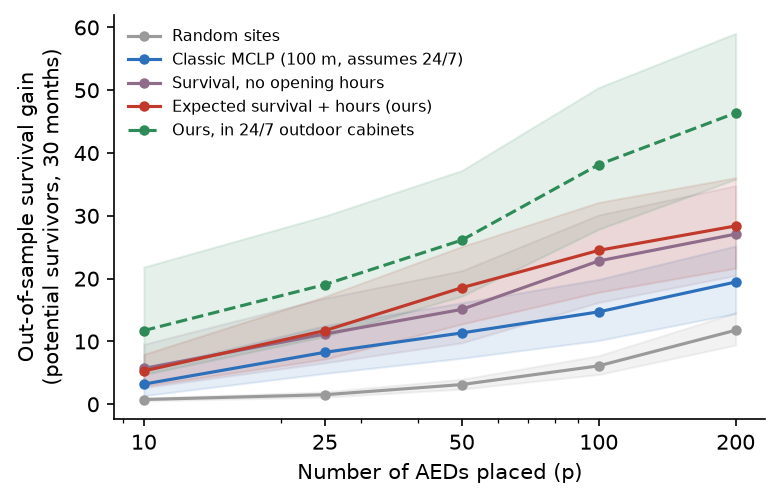
\includegraphics[width=0.62\linewidth]{fig4_cross_validation.png}
\caption{Out-of-sample expected survival gain with 95\% address-clustered bootstrap bands. The dashed line is our model with every AED in a 24/7 outdoor cabinet.}
\label{fig:cv}
\end{figure}

\begin{figure}[htbp]
\centering
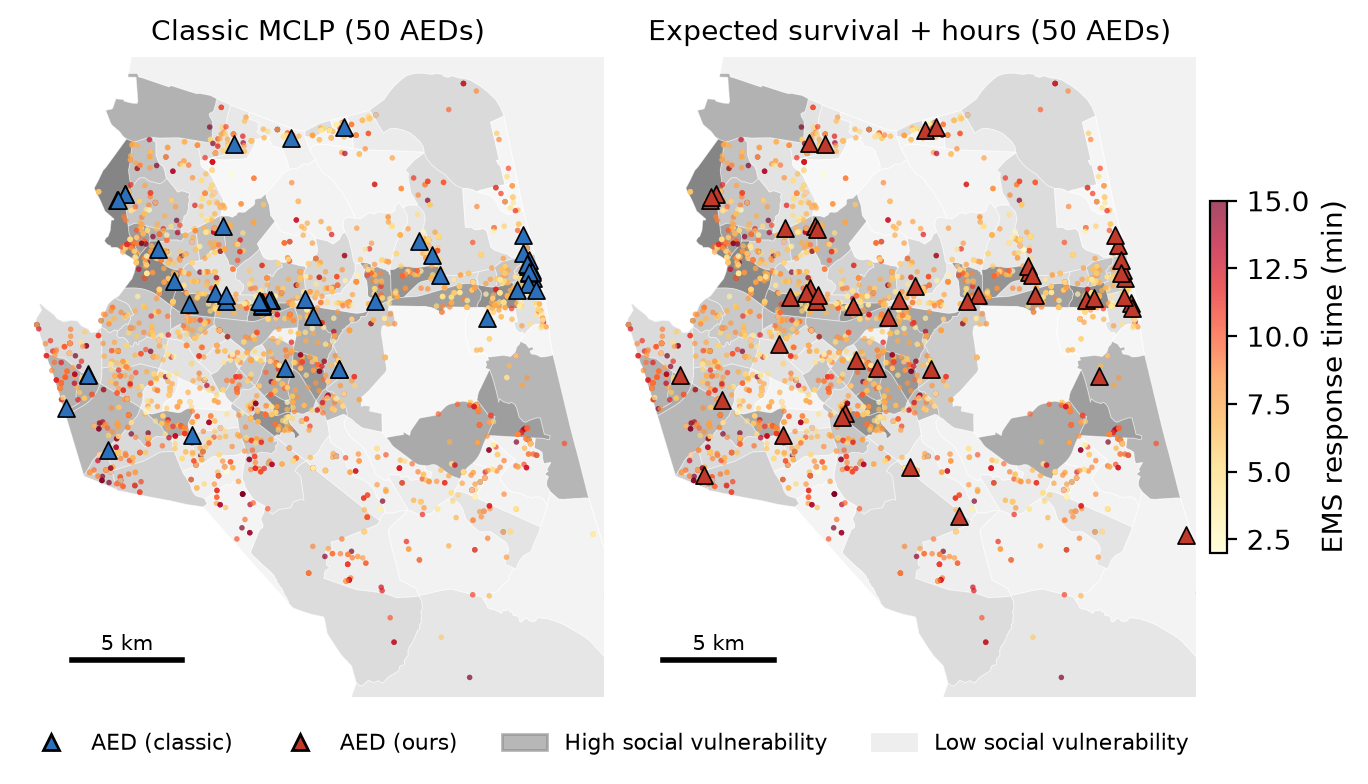
\includegraphics[width=\linewidth]{fig3_map.png}
\caption{Fifty AED sites chosen by the classic MCLP (left) and by our model (right), trained on 2017--18. Dots are cardiac arrests colored by EMS response time; tract shading is the Social Vulnerability Index. Blank areas had no recorded arrests in the study period.}
\label{fig:map}
\end{figure}

\subsection{RQ2: opening hours matter more than expected}

\begin{table}[htbp]
\centering\small
\begin{tabular}{rcccc}
\toprule
$p$ & Promised by hours-blind plan & Delivered by that plan & Hours-aware (ours) & Ours in cabinets\\
\midrule
25  & 19.1 & 11.2 & 11.7 & 19.1\\
50  & 26.1 & 15.1 & 18.6 & 26.1\\
100 & 38.2 & 22.8 & 24.5 & 38.2\\
200 & 46.4 & 27.1 & 28.4 & 46.4\\
\bottomrule
\end{tabular}
\caption{Out-of-sample expected survival gain (potential survivors) when planners ignore or use opening hours. Without opening hours, our model is the same as the cabinet model, so the hours-blind plan's promise is exactly what it would deliver if its AEDs were in 24/7 cabinets.}
\label{tab:hours}
\end{table}

Treating indoor host facilities as accessible around the clock introduces large optimism bias into AED planning. On held-out arrests, a plan that ignores opening hours promises 67--73\% more benefit than it delivers at $p=25$--$200$ (106\% at $p=10$) (Table~\ref{tab:hours}, Figure~\ref{fig:hours}). This is well above the 21.5\% overstatement documented in Toronto \cite{sun2016}. Building opening hours into the placement model recovers part of that gap: 23\% more delivered benefit at $p=50$ and 7\% at $p=100$, both statistically significant. The much larger lever is the cabinet itself. Installing the same model's AEDs in secure outdoor 24/7 cabinets delivers 41--63\% more benefit than indoor placement at $p=25$--$200$.

The temporal penalty is concentrated at night: between midnight and 3 a.m., an indoor-only deployment captures only about one-fifth of the benefit of outdoor cabinets, and between 3 and 6 a.m.\ almost none. Figure~\ref{fig:reach} (right) turns this into a simple rule. Twenty-five cabinets deliver about as much as fifty indoor AEDs (19.1 vs.\ 18.6), and 100 cabinets beat 200 indoor AEDs (38.2 vs.\ 28.4). A 24/7 cabinet is therefore worth roughly \emph{two} indoor AEDs, which gives a city a break-even price without needing any cost data.

\begin{figure}[htbp]
\centering
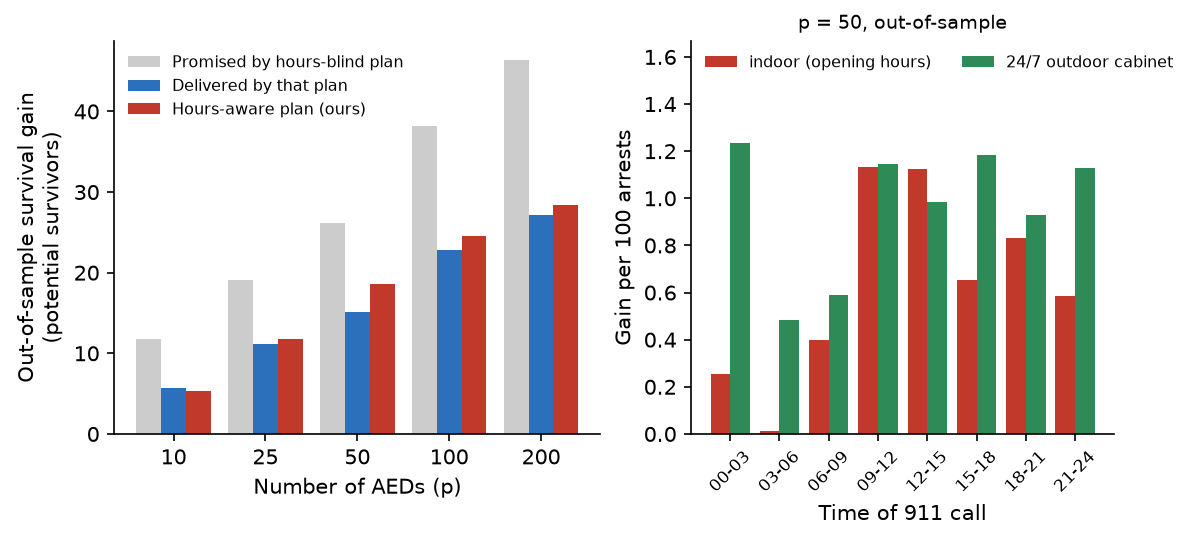
\includegraphics[width=\linewidth]{fig5_opening_hours.png}
\caption{\textbf{Left:} out-of-sample benefit an hours-blind AED plan promises versus what it delivers, and what an hours-aware plan delivers. \textbf{Right:} out-of-sample benefit by time of the 911 call for 50 AEDs, indoors versus in 24/7 outdoor cabinets.}
\label{fig:hours}
\end{figure}

\begin{figure}[htbp]
\centering
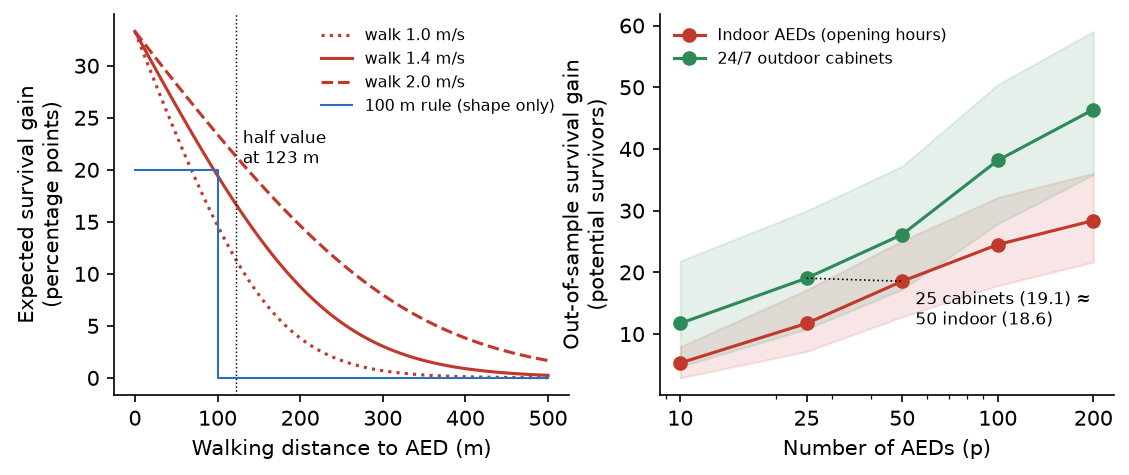
\includegraphics[width=\linewidth]{fig8_reach_cabinets.png}
\caption{\textbf{Left:} the reach curve $\rho(d)$, the expected survival gain from an AED at walking distance $d$, averaged over Virginia Beach's real EMS response times, for three walking speeds. The blue step shows the shape of the classic 100 m rule (its height is arbitrary). \textbf{Right:} out-of-sample benefit of indoor AEDs (with opening hours) versus 24/7 outdoor cabinets, with 95\% bands.}
\label{fig:reach}
\end{figure}

\subsection{RQ3: steering AEDs toward slow-EMS areas does not help}
\label{sec:rq3}
Our first model gave more weight to arrests where EMS had been slow, by using each arrest's own response time. An ablation study (Table~\ref{tab:ablation}) tests whether that ingredient matters, by comparing it with a single citywide median time and with the full response-time distribution (our main model).

\begin{table}[htbp]
\centering\small
\begin{tabular}{lccc}
\toprule
Variant (all use survival scoring and opening hours) & $p=25$ & $p=50$ & $p=100$\\
\midrule
\emph{Each arrest's own} response time & 13.3 & 17.3 & 24.0\\
\emph{Median} response time for every arrest & 12.2 & 19.9 & 24.7\\
Response time \emph{distribution} (main model) & 11.7 & 18.6 & 24.5\\
\bottomrule
\end{tabular}
\caption{Ablation: out-of-sample potential survivors. None of the pairwise differences is statistically significant (address-clustered 95\% CIs all include zero).}
\label{tab:ablation}
\end{table}

Using each arrest's own response time does \emph{not} improve out-of-sample results: the three variants are statistically indistinguishable at every budget. A location-smoothed response time (a 1 km kernel average built from training data only) did not help either. The reason is that EMS delay in Virginia Beach is barely predictable from location: a leave-one-out kernel average of nearby response times explains at most 7\% of the variance ($R^2=0.07$ at 1 km bandwidth). Delay depends far more on circumstances (which crew is free, traffic) than on place. Clinical studies show that the benefit of a bystander AED is larger when EMS is slow \cite{pollack2018,hindborg2025}, but our results suggest that, at least in this city, historical delays cannot tell a planner \emph{where} that delay will strike next.

This negative result has a positive use. If delay is essentially random with respect to place, the right planning model averages over it, which gives the reach curve $\rho(d)$ (Figure~\ref{fig:reach}, left). In Virginia Beach, an AED right next to a collapse adds about 33 percentage points of survival probability for a witnessed shockable arrest. That value \emph{halves within about 123 m of walking}, falls to 9\% of its maximum at 300 m, and is almost zero by 500 m. This explains why the common 100 m guideline is roughly the right scale, and also why a hard cutoff is wrong: it gives full credit at 99 m and none at 101 m. What drives the improvement over the classic model is the \emph{combination} of this smooth distance decay with opening hours (Table~\ref{tab:cv}). Survival scoring values the 100--250 m range that the classic model ignores, and opening hours make sure those walks lead to an AED that is actually reachable.

\subsection{RQ4: fairness is cheap, but full parity is impossible}
Without any constraint, the worst-served groups are the two \emph{least} vulnerable quartiles, not the most vulnerable one (Figure~\ref{fig:fair}). $Q_2$ was the worst served at $p=25$ and $p=50$, and $Q_1$ at $p=100$. These quartiles contain the city's low-density suburbs and its large rural south. $Q_2$ covers 474 km$^2$ with only 0.65 candidate sites per km$^2$, and $Q_1$ has 0.88 per km$^2$ and the slowest EMS (median 7.7 minutes). The two most vulnerable quartiles have about 3.0 sites per km$^2$. The most vulnerable quartile ($Q_4$) received above-average benefit at $p=50$ and $p=100$, though not at $p=25$. In Virginia Beach, AED access is a geography problem more than an income problem, unlike in England \cite{brown2025}.

Fairness is cheap. In-sample, requiring every quartile to receive at least 90\% of the citywide average costs 0.1\% of total benefit at $p=50$ and 2.6\% at $p=25$; 95\% costs 0.9\% at $p=50$. Out-of-sample, the cost was undetectable. At $p=50$, a floor of $\varphi=0.85$ raised the worst-served quartile from 0.46 to 0.62 expected survivors per 100 arrests, left the most vulnerable quartile essentially unchanged (0.80 vs.\ 0.79), and total benefit was if anything slightly higher (19.7 vs.\ 18.6).

But full parity is impossible. With an AED at every candidate site, $Q_1$ could receive at most $C_1=0.0123$ per arrest, while the all-sites citywide average is $T_\infty=0.0153$. By the Proposition, no quartile can be guaranteed more than $0.0123/0.0153\approx 81\%$ of that best-possible citywide level, whatever the budget. For a fixed budget the bound is $C_1/T_p$. At $p=100$ this is $0.0123/0.0138\approx 0.89$, and the solver found $\varphi=0.85$ feasible and $\varphi=0.90$ infeasible, consistent with the bound. At $p=25$ and $p=50$ the bound is above 1, so there the budget, not geography, is what limits fairness.

\begin{figure}[htbp]
\centering
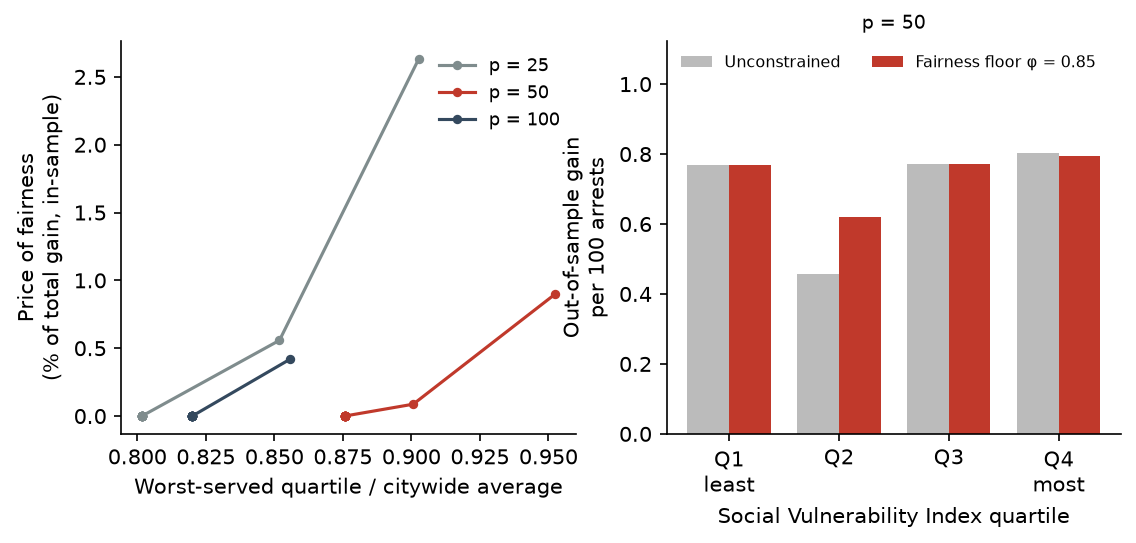
\includegraphics[width=\linewidth]{fig6_fairness.png}
\caption{\textbf{Left:} in-sample price of fairness as the worst-served quartile is raised toward the citywide average. \textbf{Right:} out-of-sample benefit per 100 arrests by SVI quartile for 50 AEDs, without and with a fairness floor.}
\label{fig:fair}
\end{figure}

\subsection{Robustness}
\label{sec:sens}
We repeated the cross-validation under ten alternative assumptions: slower (1.0 m/s) and faster (2.0 m/s) bystanders, 300 m and 800 m walking limits, the De Maio survival curve, a 2-minute call delay, a 1.5-minute AED setup time, a 2-minute EMS arrival-to-shock time, removing the 374 imputed response times, and removing the 20 most frequent addresses (which include healthcare facilities). Our model beat the classic MCLP in all 30 scenario-and-budget combinations ($p=25$, 50, 100), and the address-clustered 95\% interval excluded zero in 28 of them (Figure~\ref{fig:sens}). Both exceptions are at $p=25$: a 300 m walking limit, and removing the top-20 addresses.

\begin{figure}[htbp]
\centering
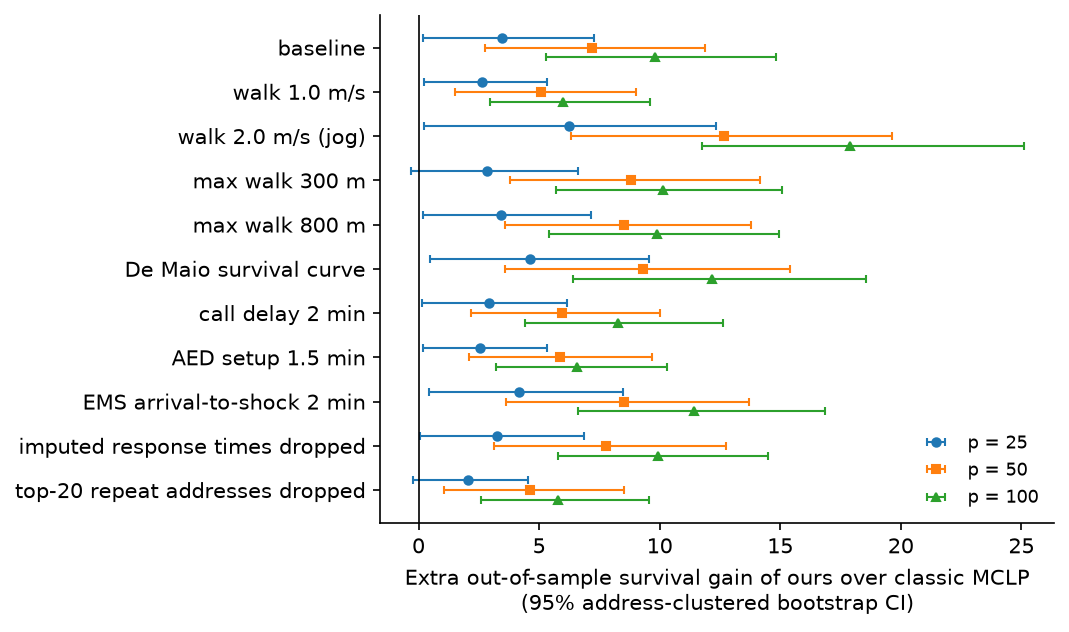
\includegraphics[width=0.7\linewidth]{fig7_sensitivity.png}
\caption{Out-of-sample advantage of our model over the classic MCLP under alternative assumptions (95\% address-clustered bootstrap intervals).}
\label{fig:sens}
\end{figure}

\section{Discussion}
\label{sec:discussion}

\paragraph{Policy guidelines for municipal AED deployment.}
Our empirical findings point to four concrete recommendations for Virginia Beach and comparable mid-sized cities.
First, building access hours are the single highest-leverage operational lever available to planners. Plans must account for them, and where possible AEDs should go in 24/7 outdoor street cabinets: on held-out arrests, 25 cabinets delivered as much expected benefit as 50 indoor units subject to closing schedules, and 100 cabinets outperformed 200 indoor units (Table~\ref{tab:hours}: 38.2 versus 28.4 potential survivors). A cabinet is worth buying whenever it costs less than about twice an indoor installation.
Second, siting optimization should evaluate walking networks with continuous survival-decay scoring rather than an arbitrary 100-meter cutoff. An AED's value halves within roughly 120 meters of walking, but walks of 100 to 250 meters still often reach patients ahead of arriving ambulances, and the classic cutoff ignores them entirely.
Third, municipal programs should avoid chasing historically slow EMS response zones. Dispatch latency in Virginia Beach is dominated by operational variance (such as crew availability and traffic) rather than persistent geographic deficits, leaving historical response times unable to guide future siting. Planners need only the city's overall response-time distribution, which most EMS agencies already publish.
Finally, cities should adopt an equity floor across social vulnerability quartiles: mandating 85--90\% parity cost at most 2.6\% of total benefit in-sample, and had no detectable cost on held-out arrests. Because commercial host buildings are scarce in low-density suburban tracts, reaching full parity will require pairing indoor units with street-side cabinets, dispatched volunteer responders, or drone delivery.

\paragraph{Estimated clinical impact.}
Translating potential survival gains into projected lives saved requires adjusting for clinical arrest presentations in the field. CARES registry data indicate that roughly 10.8\% of non-traumatic OHCAs nationwide are bystander-witnessed with a shockable rhythm \cite{caresall}. Applying this benchmark to the out-of-sample results, a deployment of 50 well-sited indoor AEDs corresponds to approximately 2.0 additional survivors across the 30-month study period (Table~\ref{tab:cv}), and housing 50 units in 24/7 outdoor cabinets raises this to approximately 2.8 (Table~\ref{tab:hours}). These figures represent practical upper bounds: even when a device is accessible, bystanders may hesitate, fail to recognize cardiac arrest, or lack retrieval assistance. Moreover, 71\% of cardiac arrests occur in private residences \cite{caresall}, beyond the reach of any fixed public AED. Public access defibrillation cannot replace baseline EMS capacity, but it serves as an indispensable multiplier during the critical early minutes of public shockable arrests.

\paragraph{Limitations and future directions.}
Several methodological constraints qualify our findings. First, the open dispatch data record 911 calls rather than confirmed cardiac arrests, omitting initial cardiac rhythms, witness status, and neurological outcomes; we therefore evaluated survival using validated logistic models from published literature \cite{valenzuela1997,demaio2003}. Second, incident addresses were rounded to the block level for privacy, and several frequent addresses represent healthcare facilities; sensitivity analyses excluding the top 20 addresses confirmed that our model still beats the classic one. Third, opening hours for 720 of the 929 candidate sites were assigned by facility category, so the size of the opening-hours effect depends on these assumed schedules; verifying the hours of the most frequently chosen sites would be the most valuable next data-collection step. Fourth, 374 missing response times were imputed via road distance to the nearest station ($r=0.21$); excluding these records did not change the ranking of methods. Fifth, our scoring assumes a single willing bystander who knows where the nearest open AED is, and starts CPR only when the AED or EMS arrives. In reality, bystander AED use remains rare \cite{cares2024}, scaling realized benefit down across all methods. Sixth, we plan from scratch and ignore any AEDs the city already has. Finally, every method is scored with the same survival model that ours optimizes; we partly guard against this by also reporting the classic 100 m coverage metric, on which our plan does not lose for $p\ge 50$.

Future investigations should link municipal spatial data directly to clinical outcomes through the CARES registry, model time-varying bystander availability using mobile mobility data, and extend the integer-programming framework to co-optimize mixed portfolios of fixed indoor units, outdoor street cabinets, and autonomous drone delivery.

\section{Prototype: AED Placement Explorer}
\label{sec:proto}
To translate our optimization framework into an operational decision tool, we developed an interactive web map application (\emph{AED Placement Explorer}, a standalone HTML/JavaScript interface in the project repository). Planners can adjust a budget slider to add AEDs sequentially in greedy order ($p=1$ to $200$) and toggle dynamically between indoor sites with empirical opening hours, 24/7 outdoor cabinets, and the classic 100-meter MCLP. The map displays all 2{,}706 cardiac arrests colored by EMS response time alongside selected host facilities, annotating each site with its operating schedule and marginal survival contribution. A telemetry sidebar reports cumulative expected survival gain, percentage improvement over the classic covering baseline, and benefit distribution across social vulnerability quartiles. The complete analytical pipeline---including data preprocessing, walking network routing, mathematical optimization, cross-validation, and figure generation---is open source and fully reproducible from public records.

\section{Conclusion}
Using only open data, we showed that an expected-survival, opening-hours-aware model places AEDs that deliver 42--67\% more expected survival gain on held-out arrests than the standard approach, and that ignoring opening hours inflates a plan's apparent benefit by roughly 70\%. A 24/7 outdoor cabinet is worth about two indoor AEDs, and an AED's value halves within about 123 m of walking. We also found that two intuitive ideas do not hold in Virginia Beach: that AEDs should follow historically slow EMS, and that the most vulnerable neighborhoods are the least served. The broader lesson is that \emph{when} an AED can be reached matters as much as \emph{where} it is, and that some gaps in access cannot be closed by placement alone.

\begin{thebibliography}{99}\small
\bibitem{cares2024} Cardiac Arrest Registry to Enhance Survival (CARES). \emph{2024 Metrics Summary}. May 2025. \url{https://mycares.net}
\bibitem{caresall} CARES. \emph{National Survival Report, 2013--2025, Non-Traumatic Etiology}. April 2026. \url{https://mycares.net}
\bibitem{larsen1993} Larsen MP, Eisenberg MS, Cummins RO, Hallstrom AP. Predicting survival from out-of-hospital cardiac arrest: a graphic model. \emph{Ann Emerg Med}. 1993;22(11):1652--1658. doi:10.1016/S0196-0644(05)81302-2
\bibitem{valenzuela1997} Valenzuela TD, Roe DJ, Cretin S, Spaite DW, Larsen MP. Estimating effectiveness of cardiac arrest interventions: a logistic regression survival model. \emph{Circulation}. 1997;96(10):3308--3313. doi:10.1161/01.CIR.96.10.3308
\bibitem{demaio2003} De Maio VJ, Stiell IG, Wells GA, Spaite DW. Optimal defibrillation response intervals for maximum out-of-hospital cardiac arrest survival rates. \emph{Ann Emerg Med}. 2003;42(2):242--250. doi:10.1067/mem.2003.266
\bibitem{erkut2008} Erkut E, Ingolfsson A, Erdo\u{g}an G. Ambulance location for maximum survival. \emph{Naval Research Logistics}. 2008;55(1):42--58. doi:10.1002/nav.20267
\bibitem{weisfeldt2010} Weisfeldt ML, Sitlani CM, Ornato JP, et al. Survival after application of automatic external defibrillators before arrival of the emergency medical system. \emph{J Am Coll Cardiol}. 2010;55(16):1713--1720. doi:10.1016/j.jacc.2009.11.077
\bibitem{pollack2018} Pollack RA, Brown SP, Rea T, et al. Impact of bystander automated external defibrillator use on survival and functional outcomes in shockable observed public cardiac arrests. \emph{Circulation}. 2018;137(20):2104--2113. doi:10.1161/CIRCULATIONAHA.117.030700
\bibitem{hindborg2025} Hindborg M, Yonis H, Gnesin F, et al. Bystander defibrillation and survival according to emergency medical service response time after out-of-hospital cardiac arrest. \emph{Prehosp Emerg Care}. 2025. doi:10.1080/10903127.2025.2478211
\bibitem{hansen2013} Hansen CM, Wissenberg M, Weeke P, et al. Automated external defibrillators inaccessible to more than half of nearby cardiac arrests in public locations during evening, nighttime, and weekends. \emph{Circulation}. 2013;128(20):2224--2231. doi:10.1161/CIRCULATIONAHA.113.003066
\bibitem{karlsson2019} Karlsson L, Malta Hansen C, Wissenberg M, et al. Automated external defibrillator accessibility is crucial for bystander defibrillation and survival. \emph{Resuscitation}. 2019;136:30--37. doi:10.1016/j.resuscitation.2019.01.014
\bibitem{deakin2018} Deakin CD, Anfield S, Hodgetts GA. Underutilisation of public access defibrillation is related to retrieval distance and time-dependent availability. \emph{Heart}. 2018;104(16):1339--1343. doi:10.1136/heartjnl-2018-312998
\bibitem{karlsson2021} Karlsson L, Sun CLF, Torp-Pedersen C, et al. Implications for cardiac arrest coverage using straight-line versus route distance to nearest automated external defibrillator. \emph{Resuscitation}. 2021;167:326--335. doi:10.1016/j.resuscitation.2021.07.014
\bibitem{toregas1971} Toregas C, Swain R, ReVelle C, Bergman L. The location of emergency service facilities. \emph{Operations Research}. 1971;19(6):1363--1373. doi:10.1287/opre.19.6.1363
\bibitem{church1974} Church R, ReVelle C. The maximal covering location problem. \emph{Papers of the Regional Science Association}. 1974;32:101--118. doi:10.1007/BF01942293
\bibitem{nemhauser1978} Nemhauser GL, Wolsey LA, Fisher ML. An analysis of approximations for maximizing submodular set functions---I. \emph{Mathematical Programming}. 1978;14:265--294. doi:10.1007/BF01588971
\bibitem{petravic2025} Petravi\'c L, Rogina KG, Mikli\v{c} R, et al. Strategic PAD positioning: a scoping review. \emph{Scand J Trauma Resusc Emerg Med}. 2025. doi:10.1186/s13049-025-01527-8
\bibitem{chan2013} Chan TC, Li H, Lebovic G, et al. Identifying locations for public access defibrillators using mathematical optimization. \emph{Circulation}. 2013;127(17):1801--1809. doi:10.1161/CIRCULATIONAHA.113.001953
\bibitem{chan2016} Chan TCY, Demirtas D, Kwon RH. Optimizing the deployment of public access defibrillators. \emph{Management Science}. 2016;62(12):3617--3635. doi:10.1287/mnsc.2015.2312
\bibitem{sun2016} Sun CLF, Demirtas D, Brooks SC, Morrison LJ, Chan TCY. Overcoming spatial and temporal barriers to public access defibrillators via optimization. \emph{J Am Coll Cardiol}. 2016;68(8):836--845. doi:10.1016/j.jacc.2016.03.609
\bibitem{sun2020} Sun CLF, Karlsson L, Morrison LJ, Brooks SC, Folke F, Chan TCY. Effect of optimized versus guidelines-based automated external defibrillator placement on out-of-hospital cardiac arrest coverage: an in silico trial. \emph{J Am Heart Assoc}. 2020;9(17):e016701. doi:10.1161/JAHA.120.016701
\bibitem{siddiq2013} Siddiq AA, Brooks SC, Chan TC. Modeling the impact of public access defibrillator range on public location cardiac arrest coverage. \emph{Resuscitation}. 2013;84(7):904--909. doi:10.1016/j.resuscitation.2012.11.019
\bibitem{pourghaderi2021} Pourghaderi AR, Kogtikov N, Lees MH, et al. Maximum expected survival rate model for public access defibrillator placement. \emph{Resuscitation}. 2021;170:213--221. doi:10.1016/j.resuscitation.2021.11.039
\bibitem{buter2024} Buter R, et al. Strategic placement of volunteer responder system defibrillators. \emph{Health Care Management Science}. 2024. doi:10.1007/s10729-024-09685-4
\bibitem{dahan2016} Dahan B, Jabre P, Karam N, et al. Optimization of automated external defibrillator deployment outdoors: an evidence-based approach. \emph{Resuscitation}. 2016;108:68--74. doi:10.1016/j.resuscitation.2016.09.010
\bibitem{aeby2021} Aeby D, Staeger P, Dami F. How to improve automated external defibrillator placement for out-of-hospital cardiac arrests: a case study. \emph{PLoS One}. 2021;16(5):e0250591. doi:10.1371/journal.pone.0250591
\bibitem{brown2025} Brown TP, Andronis L, El-Banna A, et al. Optimisation of the deployment of automated external defibrillators in public places in England. \emph{Health Soc Care Deliv Res}. 2025;13(5). doi:10.3310/HTBT7685
\bibitem{sasson2012} Sasson C, Magid DJ, Chan P, et al. Association of neighborhood characteristics with bystander-initiated CPR. \emph{N Engl J Med}. 2012;367(17):1607--1615. doi:10.1056/NEJMoa1110700
\bibitem{starks2017} Starks MA, Schmicker RH, Peterson ED, et al. Association of neighborhood demographics with out-of-hospital cardiac arrest treatment and outcomes. \emph{JAMA Cardiol}. 2017;2(10):1110--1118. doi:10.1001/jamacardio.2017.2671
\bibitem{leung2021} Leung KHB, Brooks SC, Clegg GR, Chan TCY. Socioeconomically equitable public defibrillator placement using mathematical optimization. \emph{Resuscitation}. 2021;166:14--20. doi:10.1016/j.resuscitation.2021.07.002
\bibitem{bertsimas2011} Bertsimas D, Farias VF, Trichakis N. The price of fairness. \emph{Operations Research}. 2011;59(1):17--31. doi:10.1287/opre.1100.0865
\bibitem{custodio2022} Custodio JESC, Lejeune MA. Spatiotemporal data set for out-of-hospital cardiac arrests. \emph{INFORMS Journal on Computing}. 2022;34(1):4--10. doi:10.1287/ijoc.2020.1022
\bibitem{flanagan2011} Flanagan BE, Gregory EW, Hallisey EJ, Heitgerd JL, Lewis B. A social vulnerability index for disaster management. \emph{J Homeland Security and Emergency Management}. 2011;8(1). doi:10.2202/1547-7355.1792. Data: CDC/ATSDR SVI 2022.
\end{thebibliography}

\end{document}
